\section{Abgrenzung zu Grid Computing}
Der Ansatz -- die Infrastruktur, Rechenleistung sowie Anwendungen oder Speicherplatz über ein Netzwerk für verschiedene Zwecke zur Verfügung zu stellen -- ist kein neuer.
Diese Idee, oder zumindest eine ähnliche, entstand schon vor mehreren Jahren mit dem Begriff \textbf{Grid Computing}.

Im folgenden Abschnitt werden einige Aspekte erläutert, die den Unterschied zwischen Cloud Computing und Grid Computing verdeutlichen.
 
\subsection{Der Begriff \glqq Grid Computing\grqq}
In \cite{grid-checklist} schlägt der Autor eine 3-Punkte-Checkliste vor, anhand deren sich ein Grid-System identifizieren lässt. Demnach ist Grid ein System, das:
\begin{enumerate}
  \item Ressourcen koordiniert, die keiner zentralisierten Kontrolle unterliegen
  \item dabei offene und allgemeine Standardprotokolle und Schnittstellen verwendet
  \item um nicht-triviale \glqq Quality of Services\grqq{} zu liefern
\end{enumerate}

Cloud Computing überschneidet sich nicht nur mit Grid Computing, es ist in der Tat aus Grid Computing entstanden und bildet dessen Rückgrad auf dem seine Infrastruktur aufbaut\cite{360-degree-compared}.

Das spezielle Problem, das dem Konzept des Grids in Wirklichkeit zugrunde liegt,
ist die koordinierte gemeinsame Nutzung von Ressourcen und das Lösen von Problemen
in einer dynamischen institutionsübergreifenden virtuellen Organisation.
Dabei ist mit \glqq gemeinsamer Nutzung\grqq{} der direkte Zugang zu Computern, Software, Daten und anderen Ressourcen,
die für das Lösen von Problemen in industriellen, wissenschaftlichen und technischen Bereichen benötigt werden, zu verstehen.
Das Teilen der Ressourcen beinhaltet klar definierte Regeln, die notwendigerweise stark kontrolliert werden.
Was geteilt werden kann, wer teilen darf und unter welchen Bedingungen geteilt werden darf ist dabei klar und sorgfältig definiert.
Eine Gruppe von Individuen und/oder Institutionen, die durch solche Regeln definiert sind,
bilden die sogenannten \textbf{Virtuellen Organisationen}.\cite{anatomy-of-grid}

\subsection{Anwendungsbereich}
Während Cloud Computing hauptsächlich Lösungen für verschiedene kommerzielle webbasierte Businessfälle bietet, wird Grid Computing dagegen mehr in wissenschaftlichen Gebieten wie Chemie, Physik, Genetik, Kryptologie und Mathematik bei rechenintensiven Aufgaben eingesetzt \cite{5623257}.

Grids stellen Rechenressourcen bereit, die zum Speichern und Analysieren von großen Datenmengen verwendet werden. Davon profitiert beispielsweise der \textbf{Large Hadron Collider} bei CERN.\cite{wlcg}

Der Zugriff auf die verschiedenen Arten von Anwendungen kann über sogenannte \textit{Scientific Gateways} bereitgestellt werden. Außerdem bieten diese Gateways die Möglichkeit zur Entdeckung von Ressourcen sowie Job-Excecution-Dienste auf die über Internetbrowser zugegriffen werden kann\cite{360-degree-compared}.
% Weiterhin findet Grid Einsatz in solchen Wissenschaftsgebieten wie 

\subsection{Geschäftsmodell}
Typischerweise ist das Geschäftsmodell der Grids (zumindest im akademischen Bereich) projektorientiert und die Anwender oder die Community hat eine bestimmte Anzahl an Serviceeinheiten, die verbraucht werden können\cite{360-degree-compared}.  
Dieses Konzept wird beispielsweise von XSEDE (Extreme Science and Engineering Discovery Environment) -- einem Anbieter von digitalen Dienstleistungen wie Supercomputern -- verwendet\cite{xsede}.
Wenn eine Institution mit ihren eigenen Ressourcen einem solchen Netzwerk beitritt stellt sie diese zur Nutzung für die Community bereit und kann auf die Ressourcen der anderen zugreifen\cite{360-degree-compared}.



\subsection{Architektur}
Die Grid-Netze konzentrieren sich auf die Integration vorhandener Ressourcen mit ihrer Hardware, Betriebssystemen, lokalem Ressourcenmanagement und der Sicherheitsinfrastruktur.
Um die Entdeckung sowie die gemeinsame Nutzung von diesen Ressourcen in den sogenannten \glqq Virtuellen Organisationen\grqq{} zu ermöglichen, stellen Grids eine Menge von Standardprotokollen, Middleware, Toolkits sowie Diensten, die auf diesen Protokollen aufbauen, bereit.
Da Ressourcen von verschiedene administrativen Domänen sein können und somit ihre eigene Verwendungsregeln, andere Hard- oder Softwarekonfiguration haben können, stellt die Interoperabilität und Sicherheit das Hauptanliegen für die Gridinfrastruktur dar.\cite{360-degree-compared}
\hl{Grid ist also schon vom Konzept her in der Lage diesen Herausforderungen stand zu halten.}\todo{evtl. Zitat}

Die Grid Architektur besteht aus fünf verschiedenen Schichten. Jede einzelne Schicht hat einen spezifischen Zweck und stellt entsprechende Protokolle bereit \cite{360-degree-compared}:

\begin{itemize}
\item \textbf{\textit{Fabric layer}} stellt Rechen-, Speicher-, Netzwerkressourcen bereit.
\item \textbf{\textit{Connectivity layer}} definiert Kommunikations- und Authentifizierungsprotokolle.
\item \textbf{\textit{Resource layer}} definiert unter anderem Protokolle zum Publizieren, Entdecken und Vermitteln von Ressourcen.
\item \textbf{\textit{Collective layer}} zum Erfassen von Interaktionen zwischen Sammlungen von Ressourcen.
\item \textbf{\textit{Application layer}} enthält Benutzeranwendungen, die auf den o.g. Protokollen aufbauen.
\end{itemize}

% In der Abbildung \ref{gvc} wird die Grid Protokollarchitektur mit der Cloud Architektur vergleichend dargestellt.

% \begin{figure}[ht]
% 	\centering
%   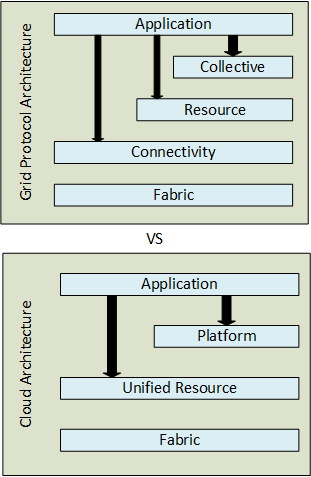
\includegraphics[width=0.4\textwidth, height=9cm]{Images/grid-vs-cloud.png}
% 	\caption{Grid Protokollarchitektur vs. Cloud Architektur}
% 	\label{gvc}
% \end{figure}



% \begin{figure}[ht]
% 	\centering
%   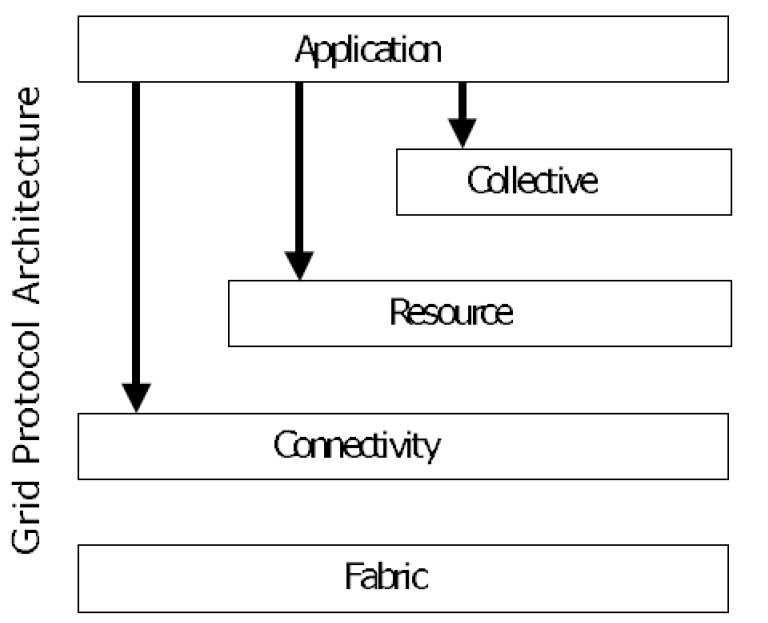
\includegraphics[width=0.5\textwidth]{Images/grid-protocol-arch.jpg}
% 	\caption{Grid Protokollarchitektur\cite{360-degree-compared}}
% 	\label{gpa}
% \end{figure}

% \begin{figure}[ht]
% 	\centering
%   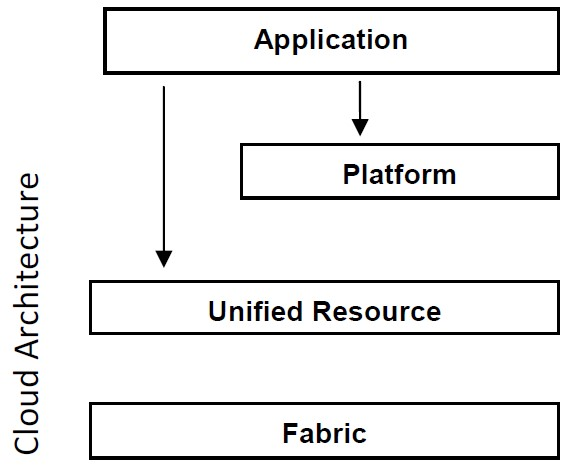
\includegraphics[width=0.3\textwidth]{Images/cloud-arch.jpg}
% 	\caption{Cloud Architektur\cite{360-degree-compared}}
% 	\label{gpa}
% \end{figure}

\subsection{Ressourcenverwaltung}
Während Grid Computing versucht Ressourcen zu bündeln, die innerhalb unterschiedlicher Organisationen sich befinden, bietet Cloud Computing diese meistens innerhalb einer einzelnen Organisation an. Dies vereinfacht unter anderem solche Aspekte wie Sicherheit, Verfügbarkeit und Heterogenität\cite{comp-cloud-grid-cluster-virt}.
Die Ressourcen einer virtuellen Organisation können geographisch verteilt sein.

Der Einsatz von Middlewareanwendungen bietet eine zusätzliche Schicht an Homogenität, um das Problem mit der heterogenen Hard- und Software etwas zu lindern. Dadurch wird die Ressourcenverwaltung innerhalb der virtuellen Organisationen vereinfacht. Jedoch bleibt die Entwicklung der Grid-übergreifenden Anwendungen, die mehrere virtuelle Organisationen betreffen immer noch schwierig.\cite{McEvoy:2008:UCA:1462704.1462715}

Grid Computing baut nicht so viel auf der Virtualisierung wie Cloud Computing, was allerdings daran liegen kann, dass jede einzelne Organisation ihre eigenen Ressourcen, die nicht notwendigerweise virtualisiert sind, selbst verwalten will\cite{360-degree-compared}. 

Aus Benutzersicht werden Ressourcen bei Cloud Computing zentral verwaltet.
Der Benutzer kann, im Web, vom Cloud Provider zur Verfügung gestellte Schnittstelle verwenden,
um Ressourcen bei Bedarf flexibel auf Anforderung hinzuzufügen oder zu entfernen.
Grid Computing ist in dieser Hinsicht dezentralisiert. Die Ressourcen können sich in unterschiedlichen virtuellen Organisationen befinden. Außerden ist eine flexible Erweiterung der Ressourcen nicht möglich. Um auf zusätzliche Ressourcen zugreifen zu können muss zuerst einer virtuellen Organisation beigetreten werden, was durch manuelle Genehmigungen eine längere Zeit dauern kann.

Während im Grid die Ressourcen meistens von einem lokalen Ressourcenmanager unter Verwendung von Batch-Scheduling verwaltet werden und die Berechnungen eins nach dem anderen abgearbeitet werden, sind in der Cloud alle Ressourcen für alle Benutzer zur gleichen Zeit verfügbar\cite{360-degree-compared}.

% \subsection{Fazit}
% \hlred{
% } 

% [Wie sieht es für die Zukunft aus?]

% \hl{Wird man in der Zukunft komplett auf Grid Computing verzichten können und stattdessen auf Cloud Computing Lösungen zugreifen?}
